\chapter{Part}
%\section{Plot the data and the autocorrelation function. Decompose your time series into trend, cycle, and seasonal component with a methodology of your choice (classical decomposition, SEATS, etc). Discuss briefly the properties of the series and the limitation of the methodology you choose (5 lines). }
\section{Plot, ACF, and Decomposition}
Figure \ref{fig:FCPI_ACFCPI} shows the French Consumer Price Index from January 1960 to December 2019 and the ACF of the french consumer price index.

The series displays a strong and persistent upward trend throughout the entire period. The growth is particularly steep during the 1970s and early 1980s, after which the rate of increase slows down noticeably. There is no sign of the series reverting to a fixed mean, which is an indication that it is non-stationary.

The ACF of the series decays very slowly and remains large and positive for many lags, well beyond the 95\% confidence bands. This is a classic sign of a non-stationary series with a trend.

\begin{figure}[H]
    \centering
    % Include the first plot image file
    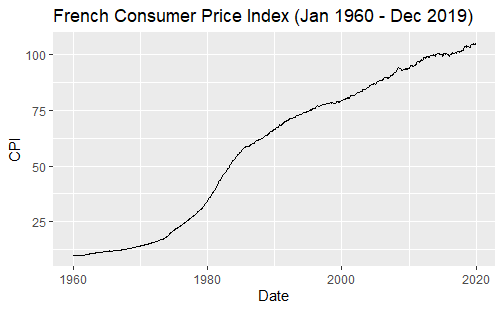
\includegraphics[width=0.45\textwidth]{billeder/French_CPI_1960-2019.png} 
    \hspace{1cm} % Add some horizontal space
    % Include the second plot image file
    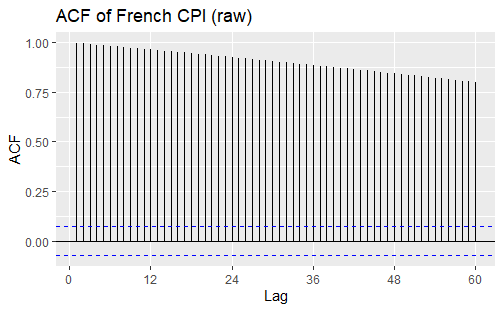
\includegraphics[width=0.45\textwidth]{billeder/ACF_of_french_CPI_raw.png}
    \caption{Figure 2: A global caption for both plots.}
    \label{fig:FCPI_ACFCPI}
\end{figure}

\textbf{Classical Decomposition}: We decompose the series into three components using classical multiplicative decomposition:
\[
\text{CPI}_t = T_t \times S_t \times R_t
\]
where $T_t$ is the trend, $S_t$ is the seasonal component, and $R_t$ is the remainder. The decomposition confirms that the trend dominates the series. The seasonal component is relatively small but present, showing a recurring pattern within each year. The remainder fluctuates randomly around one.

\begin{figure}[H]
    \centering
    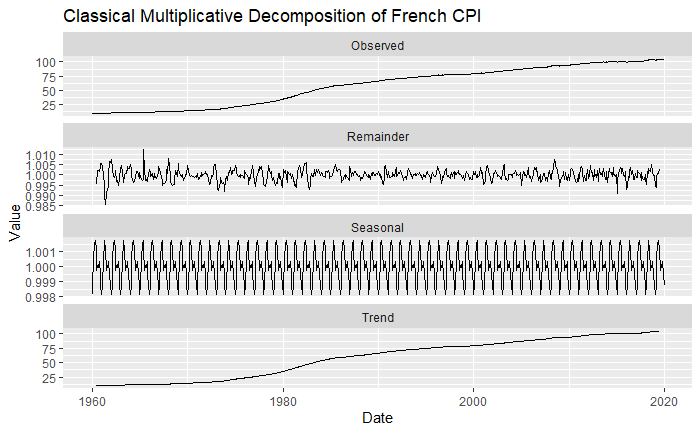
\includegraphics[width=0.7\linewidth]{billeder/Classical_Multipliacative_decomposition_of_french_CPI_2.png}
    \caption{Component graphs from classical decomposition}
    \label{fig:placeholder}
\end{figure}

\textbf{Limitations}: Classical decomposition uses a centred moving average to estimate the trend, which means the first and last six months of the series have no trend estimate. Second, it assumes that the seasonal pattern is the same every year across the full 60-year sample, which is unlikely to hold in practice. Third, the method does not separate a cyclical component from the trend, so any medium-term cycles are absorbed into the trend estimate.



%\section{Transform your data by taking natural logarithm or with Box and Cox methodology. Repeat the analysis of point 1.1: how does it change? Decide whether to use original or transformed data in the rest of the assignment. Motivate your choice.  }
\section{Log Transformation and Comparison}
We transform the CPI series by taking the natural logarithm:
\[
y_t = \log(\text{CPI}_t)
\]
\begin{figure}[H]
    \centering
    % Include the first plot image file
    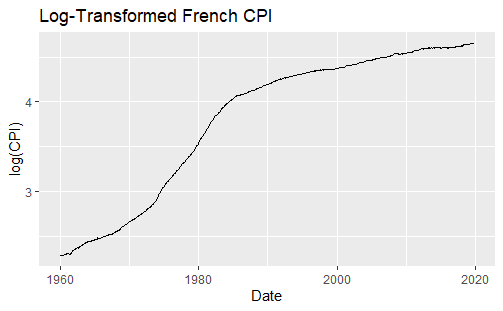
\includegraphics[width=0.45\textwidth]{billeder/Log_transformed_French_CPI.png} 
    \hspace{1cm} % Add some horizontal space
    % Include the second plot image file
    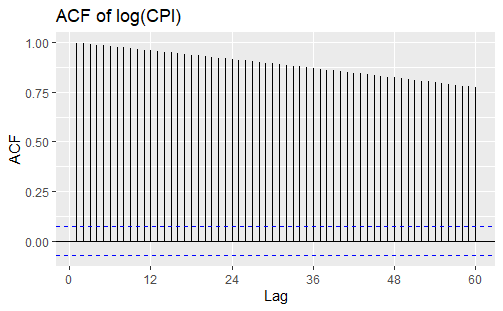
\includegraphics[width=0.45\textwidth]{billeder/ACF_of_log_CPI.png}
    \caption{Figure 2: A global caption for both plots.}
    \label{fig:two_plots}
\end{figure}

\textbf{Comparison with the Raw Series}: In the raw series, the seasonal swings and short-run fluctuations grow noticeably larger as the CPI level rises. After taking logs, these fluctuations become roughly constant in size across the full sample.

The ACF of the log-transformed series looks very similar to the ACF of the raw series - it decays slowly and stays above the confidence bands for many lags. This confirms that the log transformation has not resolved the non-stationarity of the series.

% The decomposition of the log-transformed series uses an additive form:

% \[
% \log(\text{CPI}_t) = T_t + S_t + R_t
% \]

% This is appropriate because once the variance is stabilised by the log, the seasonal component no longer needs to scale with the trend.

\textbf{Decision going forward}: We use the log-transformed series $\log(\text{CPI}_t)$ for all remaining analyses. The transformation stabilises the variance without changing the structure of the series, and working in logs means that first differences can be interpreted as approximate month-on-month percentage changes in the price level, which is economically meaningful.



%\section{Based on the results in point 1.1 and the choice in point 1.2, discuss what is the most accurate functional form for the KPSS and ADF tests. Then, perform both tests to check stationarity and discuss the results.  }
\section{Stationarity Tests}

Based on the plots and decomposition in Parts 1.1 and 1.2, $\log(\text{CPI}_t)$ has a clear upward trend throughout the sample. This means the most appropriate functional form for both tests must include a trend term. Omitting the trend would misspecify the tests, since a trending series will look non-stationary for the wrong reason. We therefore use the following specifications:

\begin{itemize}
    \item \textbf{ADF}: include a constant and a linear trend. The null hypothesis is that the series has a unit root.
    \item \textbf{KPSS}: test for stationarity around a deterministic trend. The null hypothesis is that the series is trend-stationary, so rejecting it means the series is not stationary even around a trend.
\end{itemize}

\textbf{ADF Test Results}: Table~\ref{tab:adf} reports the ADF test statistic and the corresponding critical values.

\begin{table}[h]
\centering
\begin{tabular}{lccc}
\hline
 & 1\% & 5\% & 10\% \\
\hline
Critical value ($\tau_3$) & $-3.96$ & $-3.41$ & $-3.12$ \\
Test statistic            & \multicolumn{3}{c}{$1.640$} \\
\hline
\end{tabular}
\caption{ADF test statistic and critical values for $\log(\text{CPI}_t)$.}
\label{tab:adf}
\end{table}

The test statistic of $1.640$ is far above all critical values. 
We therefore conclude that $\log(\text{CPI}_t)$ is non-stationary at all conventional significance levels.

\textbf{KPSS Test Results}: The KPSS test gives a test statistic of $2.463$ with a $p$-value of $0.01$. Since the $p$-value is below $0.05$, we reject the null hypothesis of trend stationarity. This confirms the conclusion from the ADF test.

% \subsection*{Conclusion}

% Both tests agree: $\log(\text{CPI}_t)$ is non-stationary. The ADF fails to reject the presence of a unit root, and the KPSS rejects stationarity around a trend. Differencing is therefore needed before an ARIMA model can be fitted.





%\section{If the series is not stationary, follow the approach presented in class to make it stationary. When the series is stationary, look at the autocorrelation and partial autocorrelation function, choose an ARIMA model for the series and write down the equation of the model in the form ARIMA(p,d,q)(P,D,Q)[m]. (Hint: if there is a deterministic trend, you need to detrend the time series).  }
\section{Making the Series Stationary and ARIMA Identification} \lab

\textbf{Regular Differencing}: Since the stationarity tests in Part 1.3 confirmed that $\log(\text{CPI}_t)$ contains a unit root, we apply a first regular difference:

\[
\Delta \log(\text{CPI}_t) = \log(\text{CPI}_t) - \log(\text{CPI}_{t-1})
\]

We then run a KPSS test for level stationarity on the differenced series. The test gives a statistic of $4.220$ with a $p$-value of $0.01$, meaning we still reject stationarity. One regular difference is therefore not enough on its own, which points to remaining seasonal non-stationarity in the series.

\textbf{Seasonal Differencing}: We apply an additional seasonal difference with a lag of 12, giving the fully differenced series:

\[
\Delta \Delta_{12} \log(\text{CPI}_t) = (1 - B)(1 - B^{12})\log(\text{CPI}_t)
\]

where $B$ is the backshift operator. This removes both the stochastic trend and the seasonal unit root, leaving a stationary series that we can use for ARIMA identification.

\textbf{Model Identification from ACF and PACF}: We inspect the ACF and PACF of the stationary series up to 48 lags to determine the appropriate ARIMA orders.

For the non-seasonal part, the ACF shows a significant spike at lag 1 that cuts off sharply afterwards, while the PACF decays gradually. This pattern is characteristic of a moving average process of order one, giving $p = 0$ and $q = 1$.

For the seasonal part, the ACF shows a significant spike at lag 12 that cuts off, while the PACF also has a spike at lag 12. This points to a seasonal moving average term of order one, giving $P = 0$, $Q = 1$, and $D = 1$ with $m = 12$.

The proposed model is therefore $\text{ARIMA}(0,1,1)(0,1,1)[12]$, also known as the Airline Model, with the following equation:

\[
(1 - B)(1 - B^{12})\log(\text{CPI}_t) = (1 + \theta_1 B)(1 + \Theta_1 B^{12})\varepsilon_t, \quad \varepsilon_t \sim \text{WN}(0, \sigma^2)
\]

\textbf{Estimation Results}: Table~\ref{tab:manual} reports the estimated coefficients from fitting the model to the full sample.

\begin{table}[h]
\centering
\begin{tabular}{lcc}
\hline
Parameter & Estimate & Std. Error \\
\hline
$\theta_1$ (MA1)  &  $0.2954$ & $0.0327$ \\
$\Theta_1$ (SMA1) & $-0.5995$ & $0.0321$ \\
\hline
$\hat{\sigma}^2$ & \multicolumn{2}{c}{$6.44 \times 10^{-6}$} \\
AIC              & \multicolumn{2}{c}{$-6445.92$} \\
\hline
\end{tabular}
\caption{Estimated coefficients for the manual ARIMA$(0,1,1)(0,1,1)[12]$ model.}
\label{tab:manual}
\end{table}

Both coefficients are precisely estimated and statistically significant. The positive non-seasonal MA coefficient ($\hat{\theta}_1 = 0.295$) suggests that a positive shock in one month is partly carried forward to the next. The negative seasonal MA coefficient ($\hat{\Theta}_1 = -0.600$) indicates a corrective pattern at the seasonal frequency, meaning that a positive shock in one month tends to be followed by a negative adjustment twelve months later.

